Below is a figure which shows the main window of the GID - pre processor and its different parts. Within the manual, references will be made to these different parts.

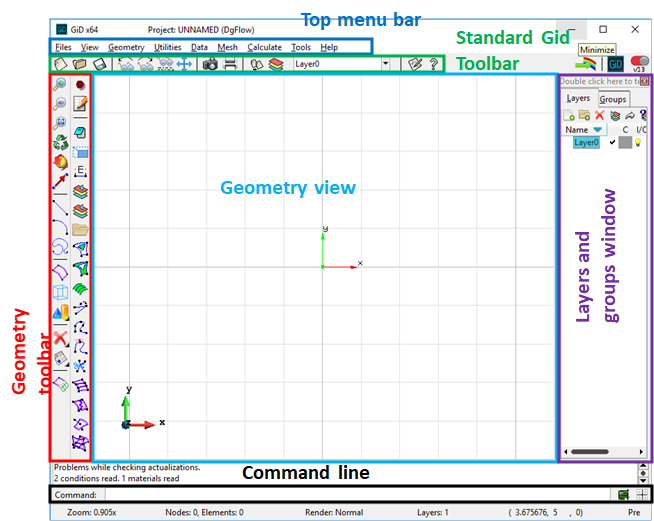
\includegraphics[width=0.9\textwidth]{GIDMainWindow.png} 



\begin{enumerate}
	\setlength\itemsep{2mm}
	
	\item Download KratosGeoMechanics from the buildserver (Deltares only) \href{https://build.deltares.nl/viewType.html?buildTypeId=GEOFEA_KratosGeo_Compile}{Download KratosGeoMechanics}. Click on the 
\includegraphics{artifactsIcon.png} icon of the latest build where all tests succeed download KratosGeoMechanics.zip.
	
	\item unzip \textbf{KratosGeoMechanics.zip} and place it in a convenient location.
	
	\item Go to \href{https://www.python.org/downloads/release/python-375/} {Download python 3.7} and download \textit{"Windows x86-64 embeddable zip file"}.
	
	\item unzip the python zip file. From the unzipped directory, copy: \textbf{"python37.dll"}. And paste it in the \textit{"KratosGeoMechanics"} directory.
	
	\item Download GID from \href{https://www.gidhome.com/download/official-versions/}{Download GID}. The problemtype is made while using GID version 14*. 
	
	\item In the KratosGeoMechanics directory go to: \newline "applications/GeoMechanicsApplication/custom$\_$problemtype/ \newline GeoMechanicsApplication.gid"
	
	\item right click and edit \textbf{"GeoMechanicsApplication.win.bat"}. Replace all the paths until \textit{"*\textbackslash\textbackslash Kratos"} with the location of the KratosGeoMechanics dir on your local drive. For example :
	replace \textit{"D:\textbackslash\textbackslash src\textbackslash\textbackslash Kratos\textbackslash\textbackslash runkratos"} by \newline \textit{"C:\textbackslash\textbackslash Users\textbackslash\textbackslash noordam\textbackslash\textbackslash Downloads\textbackslash\textbackslash KratosGeoMechanics\textbackslash\textbackslash runkratos"}. Note that the double backslashes are required for path separations.
		
	\item Copy the \textbf{GeoMechanicsApplication.Gid} problemtype paste it in the GiD problemtypes folder, e.g. : \textit{C:/Program Files/GiD/GiD 14.0.3/problemtypes/} 
	
	\begin{itemize}
		\setlength\itemsep{2mm}
		\item \textit{When performing this step, GID files can easily be transferred between different PC’s, however admin rights on your computer are required for this step.}
		
		\item  \textit{If you do not have admin rights, it is still possible to use GID and to transfer GID files between different PC’s, however, more effort is required to retain all data. Explanation is given in section @@@.}
	\end{itemize}
	
	\item Open GiD (it is recommended to have your GiD window on your main screen, since GiD pop-up messages appear on your main screen)
	
	\item If you performed Step 8, perform Step 10.1, else perform Step 10.2. 
	\begin{enumerate}
		\item In the top menu bar choose: Data ->  Problem type-> GeoMechanicsApplication
		
		\item In the top menu bar choose: Data ->  Problem type-> Load…  and choose file: \textit{GeoMechanicsApplication.gid} from any locations  	
	\end{enumerate}
	\item In the top menu bar choose:  Utilities ->  Preferences.
	\item In the Preferences window choose: Grid
	\begin{itemize}
		\setlength\itemsep{2mm}
		\item Alter the domain size to your liking (X Extents / Y Extends)
		\item In General options: activate the options as preferred.
		\item In Spacing: alter the spacing for which your pointer snaps to a location.
	\end{itemize}

	
\end{enumerate}

